\documentclass[tikz,border=0pt]{standalone}
% Shared visual language for every block diagram in figures/diagrams.
% Build with XeLaTeX (see figures/diagrams/build.sh).
\usepackage{fontspec}
\setmainfont{Inter}[Numbers=Lining]
\setmonofont{DejaVu Sans Mono}[Scale=0.86]
\usepackage{xcolor}
\usetikzlibrary{arrows.meta,positioning,calc,fit,backgrounds,shapes.geometric,
  shapes.misc,matrix,decorations.pathreplacing,patterns,quotes}

% Palette (matches python/figstyle.py) --------------------------------------
\definecolor{surface}{HTML}{FCFCFB}
\definecolor{ink}{HTML}{0B0B0B}
\definecolor{ink2}{HTML}{52514E}
\definecolor{muted}{HTML}{898781}
\definecolor{hair}{HTML}{E1E0D9}
\definecolor{memline}{HTML}{2A78D6}  \definecolor{memfill}{HTML}{E7F0FC}
\definecolor{aluline}{HTML}{14875E}  \definecolor{alufill}{HTML}{E3F5EE}
\definecolor{ctlline}{HTML}{B07800}  \definecolor{ctlfill}{HTML}{FDF2D9}
\definecolor{regline}{HTML}{6250D6}  \definecolor{regfill}{HTML}{ECEAFB}
\definecolor{wire}{HTML}{3D3C39}
\definecolor{accent}{HTML}{EB6834}   \definecolor{accentfill}{HTML}{FDE8DF}
\definecolor{pos}{HTML}{E34948}      \definecolor{posfill}{HTML}{FBE1E0}
\definecolor{neg}{HTML}{2A78D6}      \definecolor{negfill}{HTML}{DCE9FA}
\definecolor{zerofill}{HTML}{F0EFEC}

\tikzset{
  every picture/.style={line cap=round, line join=round, font=\small, text=ink},
  % canvas
  canvas/.style={show background rectangle,
    background rectangle/.style={fill=surface, draw=hair, rounded corners=8pt, line width=0.6pt},
    inner frame xsep=16pt, inner frame ysep=14pt},
  ttl/.style={font=\bfseries\large, anchor=north west, inner sep=0pt, text=ink},
  sub/.style={font=\small, anchor=north west, inner sep=0pt, text=ink2},
  % blocks
  blk/.style={rounded corners=3pt, line width=0.8pt, align=center, minimum height=9mm,
    inner xsep=5pt, inner ysep=3pt},
  mem/.style={blk, draw=memline, fill=memfill},
  alu/.style={blk, draw=aluline, fill=alufill},
  ctl/.style={blk, draw=ctlline, fill=ctlfill},
  reg/.style={blk, draw=regline, fill=regfill, rounded corners=1pt},
  io/.style={blk, draw=muted, fill=white},
  ghost/.style={blk, draw=muted, dashed, fill=surface},
  % arithmetic primitives
  add/.style={circle, draw=aluline, fill=white, line width=0.8pt, minimum size=6.2mm,
    inner sep=0pt, font=\normalsize},
  shf/.style={rectangle, rounded corners=1.5pt, draw=aluline, fill=white, line width=0.7pt,
    font=\ttfamily\footnotesize, inner xsep=2.5pt, inner ysep=2pt, minimum height=5mm},
  gain/.style={isosceles triangle, isosceles triangle apex angle=60, draw=aluline, fill=white,
    line width=0.7pt, inner sep=1.2pt, font=\footnotesize},
  dn/.style={circle, draw=wire, fill=white, line width=0.7pt, minimum size=8mm, inner sep=0pt,
    font=\footnotesize},
  mux/.style={trapezium, trapezium angle=72, shape border rotate=270, draw=ctlline, fill=ctlfill,
    line width=0.8pt, minimum height=13mm, minimum width=5mm, inner sep=1pt, font=\scriptsize},
  net/.style={draw=memline, fill=memfill, rounded corners=1.5pt, font=\footnotesize, inner xsep=3pt,
    inner ysep=1.6pt, minimum width=5.5mm, minimum height=4.8mm},
  % wires
  sig/.style={-{Latex[length=2.2mm,width=1.6mm]}, draw=wire, line width=0.75pt},
  bus/.style={-{Latex[length=2.6mm,width=2mm]}, draw=wire, line width=1.5pt},
  ctrl/.style={-{Latex[length=1.8mm,width=1.4mm]}, draw=ctlline, line width=0.65pt, dash pattern=on 3pt off 2pt},
  nohead/.style={-, draw=wire, line width=0.75pt},
  dot/.style={circle, fill=wire, inner sep=0pt, minimum size=3.2pt},
  % labels
  lbl/.style={font=\footnotesize, text=ink2, fill=surface, inner sep=1.2pt},
  lblc/.style={font=\footnotesize, text=ink2, inner sep=1.2pt},
  note/.style={font=\footnotesize, text=ink2, align=left, inner sep=0pt},
  head/.style={font=\bfseries\small, text=ink, inner sep=0pt},
  code/.style={font=\ttfamily\footnotesize, text=ink},
  group/.style={draw=hair, fill=white, rounded corners=6pt, line width=0.8pt, inner sep=7pt},
  grouplabel/.style={font=\bfseries\footnotesize, text=muted, anchor=south west, inner sep=2pt},
}

% Layers: groups sit above the canvas background and below the main layer.
\pgfdeclarelayer{groups}
\pgfsetlayers{background,groups,main}

% A register: box with a clock wedge at the bottom edge.
\newcommand{\clk}[1]{\draw[regline, line width=0.6pt] ($(#1.south)+(-1.4mm,0)$) -- ($(#1.south)+(0,1.6mm)$) -- ($(#1.south)+(1.4mm,0)$);}
% Bus width tick: \bw{(point)}{width}
\newcommand{\bw}[2]{\draw[wire, line width=0.6pt] ($#1+(-0.9mm,-1.2mm)$) -- ($#1+(0.9mm,1.2mm)$); \node[font=\scriptsize, text=ink2, above=0.4mm, inner sep=0.5pt] at #1 {#2};}
\newcommand{\var}[1]{\textit{#1}}
\newcommand{\usub}[1]{\ifcase#1 ₀\or ₁\or ₂\or ₃\or ₄\or ₅\fi}
\AtBeginDocument{\hyphenpenalty=10000\exhyphenpenalty=10000}

\begin{document}
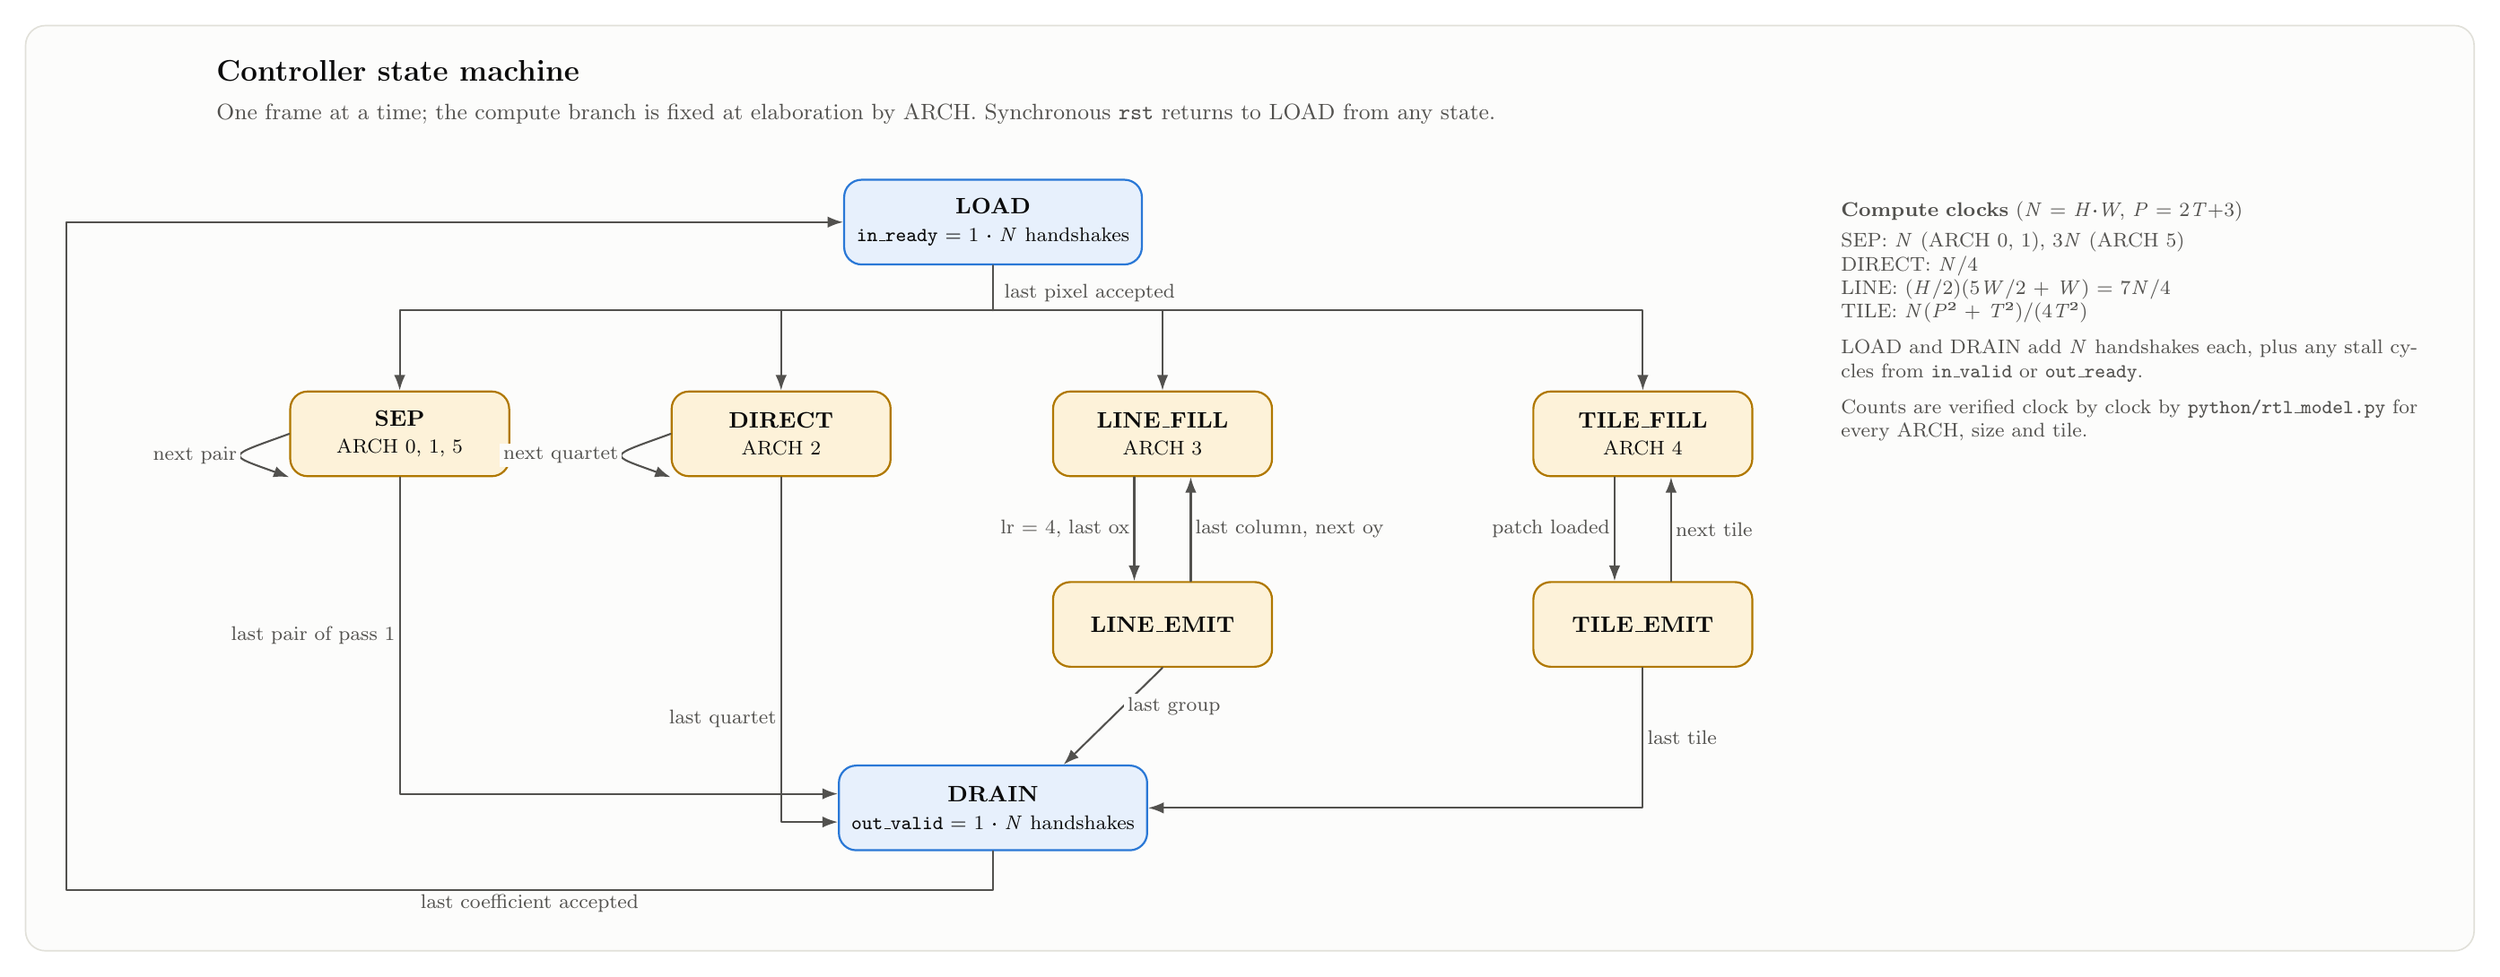
\begin{tikzpicture}[canvas]
  \node[ttl] at (0,0) {Controller state machine};
  \node[sub] at (0,-0.62) {One frame at a time; the compute branch is fixed at elaboration by ARCH. Synchronous \texttt{rst} returns to LOAD from any state.};
  \tikzset{st/.style={ctl, rounded corners=7pt, minimum width=31mm, minimum height=12mm, align=center},
           io2/.style={mem, rounded corners=7pt, minimum width=36mm, minimum height=12mm, align=center},
           tr/.style={sig, draw=ink2}, tl/.style={font=\footnotesize, text=ink2, fill=surface, inner sep=1.5pt}}
  \node[io2] (load) at (11.0,-2.3) {\textbf{LOAD}\\\footnotesize \texttt{in\_ready} = 1 · \var{N} handshakes};
  \node[st] (sep) at (2.6,-5.3) {\textbf{SEP}\\\footnotesize ARCH 0, 1, 5};
  \node[st] (dir) at (8.0,-5.3) {\textbf{DIRECT}\\\footnotesize ARCH 2};
  \node[st] (lf) at (13.4,-5.3) {\textbf{LINE\_FILL}\\\footnotesize ARCH 3};
  \node[st] (tf) at (20.2,-5.3) {\textbf{TILE\_FILL}\\\footnotesize ARCH 4};
  \node[st] (le) at (13.4,-8.0) {\textbf{LINE\_EMIT}};
  \node[st] (te) at (20.2,-8.0) {\textbf{TILE\_EMIT}};
  \node[io2] (drain) at (11.0,-10.6) {\textbf{DRAIN}\\\footnotesize \texttt{out\_valid} = 1 · \var{N} handshakes};
  \coordinate (fan) at (11.0,-3.55);
  \draw[nohead, draw=ink2] (load.south) -- (fan);
  \node[tl, anchor=west] at ($(fan)+(0.1,0.25)$) {last pixel accepted};
  \foreach \s in {sep,dir,lf,tf} \draw[tr] (fan) -| (\s.north);
  \draw[tr] (sep.west) to[out=200, in=160, looseness=4] node[tl, left] {next pair} (sep.south west);
  \draw[tr] (dir.west) to[out=200, in=160, looseness=4] node[tl, left] {next quartet} (dir.south west);
  \draw[tr] ($(lf.south)+(-0.4,0)$) -- node[tl, left] {lr = 4, last ox} ($(le.north)+(-0.4,0)$);
  \draw[tr] ($(le.north)+(0.4,0)$) -- node[tl, right] {last column, next oy} ($(lf.south)+(0.4,0)$);
  \draw[tr] ($(tf.south)+(-0.4,0)$) -- node[tl, left] {patch loaded} ($(te.north)+(-0.4,0)$);
  \draw[tr] ($(te.north)+(0.4,0)$) -- node[tl, right] {next tile} ($(tf.south)+(0.4,0)$);
  \draw[tr] (sep.south) |- node[tl, pos=0.25, left] {last pair of pass 1} ($(drain.west)+(0,0.2)$);
  \draw[tr] (dir.south) |- node[tl, pos=0.35, left] {last quartet} ($(drain.west)+(0,-0.2)$);
  \draw[tr] (le.south) -- node[tl, right, pos=0.4] {last group} ($(drain.north)+(1.0,0)$) ;
  \draw[tr] (te.south) |- node[tl, pos=0.25, right] {last tile} (drain.east);
  \draw[tr] (drain.south) -- ++(0,-0.55) -| node[tl, pos=0.25, below] {last coefficient accepted} ($(load.west)+(-11.0,0)$) -- (load.west);
  \node[note, anchor=north west, text width=8.4cm] at (23.0,-2.0) {%
    \textbf{Compute clocks} (\var{N} = \var{H}·\var{W}, \var{P} = 2\var{T}+3)\\[3pt]
    SEP: \var{N} (ARCH 0, 1), 3\var{N} (ARCH 5)\\
    DIRECT: \var{N}/4\\
    LINE: (\var{H}/2)(5\var{W}/2 + \var{W}) = 7\var{N}/4\\
    TILE: \var{N}(\var{P}² + \var{T}²)/(4\var{T}²)\\[5pt]
    LOAD and DRAIN add \var{N} handshakes each, plus any stall cycles from \texttt{in\_valid} or \texttt{out\_ready}.\\[5pt]
    Counts are verified clock by clock by \texttt{python/rtl\_model.py} for every ARCH, size and tile.};
\end{tikzpicture}
\end{document}
